\begin{center}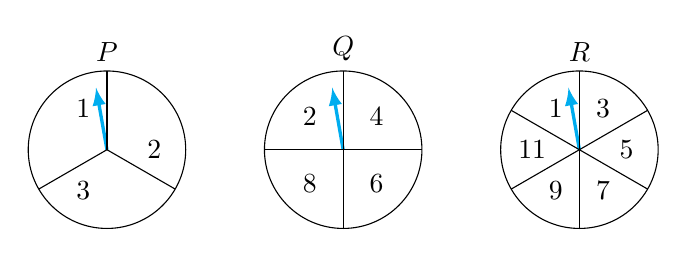
\begin{tikzpicture}[scale=1]
\foreach \p/\k/\m/\n/\r/\t/\s in {0/3/1/2/3/120/P,3/4/2/4/8/135/Q,6/6/1/3/11/120/R}{
\begin{scope}[shift={(\p,0)}]{
\draw(0,0)circle(1);
\node[above]at(0,1){ $\s$ };
\draw[very thick,-latex,cyan](0,0)--(100:0.8);
\foreach \x in {1,...,\k}{
\draw(0,0)--({90-(\x-1)*360/\k}:1);}
\foreach \x in {\m,\n,...,\r}{
\node at({\t-((\x-\m)/(\n-\m))*360/\k}:0.6){ $\x$ };
}}
\end{scope}}
\end{tikzpicture}\end{center}
